\documentclass{beamer}


\usepackage[frenchb]{babel}

\usepackage[T1]{fontenc}
%\usepackage[latin1]{inputenc}
\usepackage[utf8]{inputenc}

\usepackage{marvosym}



\newcommand{\be}[1]{ \begin{equation} \label{#1}}
\newcommand{\ee}{\end{equation}}


\newcommand{\bes}[1]{ \begin{equation} \label{#1}\begin{array}{rl}}
\newcommand{\ees}{\end{array}\end{equation}}


\usepackage[normalem]{ ulem }
\usepackage{soul}

% \usetheme{default} -> A utiliser dans un premier temps

% \usetheme{Warsaw} -> A utiliser dans un second temps


\usepackage{amsmath} % AMS Math Package
\usepackage{amsthm} % Theorem Formatting
\usepackage{amssymb} % Math symbols such as \mathbb
\usepackage{graphicx} % Allows for eps images
\usepackage{multicol} % Allows for multiple columns
\usepackage[dvips,letterpaper,margin=1in,bottom=1in]{geometry}
\usepackage{hyperref}
\usepackage{mathrsfs}
\usepackage{amsmath,amscd}
\usepackage[all,cmtip]{xy}
\usepackage{bbm}
%%%%%%%%%%%%%%%%%%%%%%%%%%%%%%%%%%%%%%%%%%%%%%%%%%%
%COLOR PACKEGE
\usepackage{color}
	\definecolor{red}{RGB}{255,0,0}
	\definecolor{blue}{RGB}{30, 144, 255}
	\definecolor{black}{RGB}{0, 0, 0}	
	\definecolor{mygreen}{RGB}{28,172,0} % color values Red, Green, Blue
	\definecolor{mylilas}{RGB}{170,55,241}
%%%%%%%%%%%%%%%%%%%%%%%%%%%%%%%%%%%%%%%%%%%%%%%%%%%
\usepackage{menukeys}
\usepackage{framed}
\renewmenumacro{\directory}{pathswithfolder} % default: paths
%%%%%%%%%%%%%%%%%%%%%%%%%%%%%%%%%%%%%%%%%%%%%%%%%%%
%MATLAB

\usepackage{listings}
\lstset{language=Matlab,%
    %basicstyle=\color{red},
	%basicstyle=\ttfamily,frame=single,xleftmargin=3em,xrightmargin=3em  
	frame=single,xleftmargin=2em,%xrightmargin=2em,    
    breaklines=true,%
    morekeywords={matlab2tikz},
    keywordstyle=\color{blue},%
    morekeywords=[2]{1}, keywordstyle=[2]{\color{black}},
    identifierstyle=\color{black},%
    stringstyle=\color{mylilas},
    commentstyle=\color{mygreen},%
    showstringspaces=false,%without this there will be a symbol in the places where there is a space
    numbers=left,%
    numberstyle={\tiny \color{black}},% size of the numbers
    numbersep=9pt, % this defines how far the numbers are from the text
    emph=[1]{for,end,break},emphstyle=[1]\color{red}, %some words to emphasise
    %emph=[2]{word1,word2}, emphstyle=[2]{style}, 
}
%%%%%%%%%%%%%%%%%%%%%%%%%%%%%%%%%%%%%%%%%%%%%%%%%%%
%\lstinputlisting{*.m} for using
%\usepackage[framed,numbered,autolinebreaks,useliterate]{mcode}
%%%%%%%%%%%%%%%%%%%%%%%%%%%%%%%%%%%%%%%%%%%%%%%%%%%
%MACROS
\newcommand{\ti}[1]{\textit{#1}}


\newcommand{\ssp}{\vspace{.2cm} }

\title{Réunion "StabFem"}

\subtitle{}

\author{D. Fabre}

\institute{IMFT, groupe Interface}

\date{6 juillet 2018}


\AtBeginSection{
\frame{\tableofcontents[current]}
}


\begin{document}


\begin{frame}

\titlepage

\end{frame}

\section{StabFem : présentation du logiciel}

%%%%%%%%%%%%%%%%%%%%%%%%%%%%%%%%%%%%%%%%%%%%%%%%
\begin{frame}{StabFem : Cahier des charges }
%Equations : 
%\begin{equation}
%$$\frac{\partial V }{\partial t} = \nu \frac{\partial^2 V}{\partial y^2} $$
%\label{eq:navier}
%\end{equation}
%(on a supposé pour simplifier qu'il n'y avait pas de gradient de pression autre qu'hydrostatique).
%Conditions limites : $\left. v\right|_{y=0} = 0$, $\left. v\right|_{y=h} = U(t)$  

\begin{itemize}[<+->]

\item StabFem : an open-source and easy-to-use software allowing a large range of computations in fluid mechanics.

\item Initially  oriented towards Global Stability Approches (Linear \& Nonlinear) but actually allowing a larger number of computations
(DNS, linear acoustics, etc...)

\item Multi-platform (Unix, MacOs, Windows) and designed to run on "light" computers (Laptops...)

\item Easy to use/install,

\item Easy to customize to a variety of cases (incompressible, compressible, fixed/free objects, free surfaces,...)

\item Freeware, based on two softwares : FreeFem++ and \sout{Matlab} %-> Octave ? Python ?

\item Developed as a collaborative project
(IMFT, Università di Salerno, ONERA, UPFL, ...)

\item Maintained on Github

\ssp
{\color{orange}
\verb! https://github.com/erbafdavid/StabFem !
}

\end{itemize}

\end{frame}





\begin{frame}{FreeFem++}

Les méthodes d'éléments finis sont bien adaptés aux problèmes de stabilité globale.

Le logiciel {\em FreeFem++} est un outil très populaire dans la communauté de la stabilité hydrodynamique.

\small

\begin{itemize}[<+->]
%{\color{green} \Smiley{} \quad }  (solides, fluides, thermique, etc...)
\item
{\color{green} \Smiley{} \quad } Syntaxe intuitive basée directement sur la formulation faible.
\item
{\color{green} \Smiley{} \quad } Mailleur puissant et adaptatif (movemesh, adaptmesh, etc...)
\item
{\color{green} \Smiley{} \quad } 2D et 3D.
\item
{\color{green} \Smiley{} \quad } Grand choix de solveurs séquentiels ou parallèles (Mumps, Petsc/Slepc, ..)
\item
{\color{red} \Frowny{} \quad } Interface graphique limitée (ffglut).
\item
{\color{red} \Frowny{} \quad } Language interprété : pas adapté à la programmation fonctionnelle (mais des macros puissantes).
\item
{\color{red} \Frowny{} \quad } Syntaxe "chatouilleuse" et débuggage parfois complexe...
\end{itemize}
\end{frame}

\begin{frame}{Pourquoi interfacer FreeFem++ avec un autre logiciel ?}

\small

\begin{itemize}[<+->]

\item Stratégie avant "StabFem" (2010-2017) :

Chaine de calcul : Solveurs FreeFem++ / Scripts Shell / Post-traitement Tecplot / Gnuplot.... 

=> 50 programmes quasiment identiques + 10 manières d'effectuer le post-traitement,

on ne s'y retrouve plus... 

\ssp 

\item Nécessité d'une surcouche "driver"  pour piloter les calculs et tracer les résultats en mode "terminal" ou par l'intermédiaire de scripts.


\item Idée (à terme) : 1 travail (1 article) = 1 unique script Matlab pour reproduire tous les calculs et générer toutes les figures 
(cf. Basilisk...)


\item Choix actuel  : Drivers en Matlab (solution non satisfaisante a terme, pb. licences...)


\end{itemize}


\end{frame}



%%%%%%%%%%%%%%%%%%%%%%%%%%%%%%%%%%%%%%%%%%%%%%%%%%%%%%%%%%%%%%%%%%%%%%%%%%
\begin{frame}{Articulation FreeFem / Matlab}

\scriptsize

\begin{itemize}[<+->]

\item 
Etage 1 : Solveurs FreeFem++ "briques de base".

Un solveur par "classe de problèmes" (2D incompressible, 2D compressible, Axisymétrique incompressible...) et par "type de calcul" (calcul d'un champ de base, stabilité linéaire, ...)


\item  Etage 2 : drivers Matlab "génériques"  

Un unique driver pour chaque "type de calcul" , le choix du bon solveur est fait en fonction 
des paramètres optionnels fournis au driver.
  

  
\item Etage 3 : Les boucles sur les paramètres et la génération des figures sont faites dans un "script principal".

\item Les solveurs et les drivers génériques sont dans des répertoires communs {\bf SOURCES\_MATLAB/} et {\bf SOURCES\_FREEFEM/}, 

\item Les programmes spécifiques à chaque cas d'étude sont dans un répertoire spécifique.

Exemple : le répertoire "CYLINDRE" contient les programmes suivants :

\begin{enumerate}
\scriptsize
\item Mesh\_Cylinder.edp		\qquad -> Génération du maillage

\item Macros\_StabFem.edp \qquad -> Macros case-dependant (conditions limites et post-traitement)   

\item SCRIPT\_CYLINDER.m $\qquad$ -> Script "Maitre".

\end{enumerate}
\end{itemize}
\pause 


{\em Remarques : les programmes FreeFem doivent pouvoir être utilisés directement en dehors du driver StabFem, 
notamment pour faciliter le développement/débuggage...)}  

\ssp 

{\em Les contributeurs "utilisateurs" (ex. étudiant M1/M2) ne travaillent qu'à l'étage 3 et ne devraient travailler que sur ces 3 fichiers.
\ssp

Les contributeurs "développeurs" travaillent aux étages inférieurs...}


\end{frame}




\begin{frame}{Format d'échange des données}

\begin{itemize}[<+->]


\item Format de fichier d'échange ".ff2m", généré par FreeFem++ et relu par Matlab
 
\item Example d'en-tête d'un fichier .ff2m :

\lstinputlisting[linerange={1-4}]{../EXAMPLE_Lshape/Data.ff2m}
 
Ligne 4 : "TypeField1 NameField1 TypeField2 NameField2... "
  
TypeField can be "real" (scalar data), "real.N" (vectorial data), "P1" (data associated to mesh), ... 

\item Le fichier est lu et importé sous forme d'une {\em structure matlab}   

\item Illustration : cas "EXAMPLE\_Lshape"

\end{itemize}


\end{frame}



\section{Using StabFem for Linear stability }


\begin{frame}{Stabilité globale : qu'es aquò ?? } 


Les problèmes d'instabilités sont omniprésents en mécanique des fluides. 

\ssp

Leur résolution fait appel à une classe de méthodes numériques spécifiques, 
complémentaires aux approches de simulation directe, qui sont actuellement en plein développement. 

\ssp

On parle {\em stabilité globale} quand la géométrie du problème necessite une résolution en 2D (ou en 3D).

\ssp

(par opposition à {\em stabilité locale} quand des directions d'invariance (écoulement parallèle par ex.) permettent de rammener le problème à une résolution en 1D).


\end{frame}

\begin{frame}{Stabilité globale : liste des types de problèmes et cas-tests}

\scriptsize

\begin{itemize}
\item CYLINDER  		\qquad -> 2D incompressible, objet fixe

\item CYLINDER\_VIV \qquad 	-> 2D incompressible, objet mobile 

(Stage Diogo Ferrera-Sabino)

\item IMPACTINGJET  		\qquad -> 2D incompressible, 3D stability.

(with David LoJacono)

\item CYLINDER\_Compressible  \qquad -> 2D compressible 

(Javier Serra, Vincenzo Citro...)

\item BIRDCALL \qquad -> 2D-axisymmetric, incompressible or "augmented incompressible"

(with R. Longobardi, V. Citro....)


\item POROUS\_DISK \qquad -> 2D-axisymmetric, with porous object 

(stage Adrien Rouvière)

\item LiquidBridges -> 2D axi, with deformable free surface

(stage Nabil Achour)

\item ROTATING\_POLYGONS

(with Jérôme Mougel...)
\item ....

\end{itemize}

=> Illustration dans le cas CYLINDER

\end{frame}


\begin{frame}{First step : Generation of a mesh and "guess" base flow}

\small

%\begin{lstlisting}
%bf=SF_Init('Mesh_Cylinder.edp', [-40 80 40]);
%\end{lstlisting}

\keys{bf=SF\_Init('Mesh\_Cylinder.edp', [-40 80 40]);}

\ssp

What the \keys{SF\_Init} driver does :

\begin{itemize}[<+->]
\item Runs the relevant FreeFem++ program \keys{Mesh\_Cylinder.edp}  with the corresponding parameters (here size of the domain),

{\scriptsize This program generates the following output files : \keys{mesh.msh} (mesh data), \keys{mesh.ff2m} (mesh information), \keys{SF\_Init.ff2m} (auxiliary information), \keys{BaseFlow\_init.txt} and \keys{BaseFlow\_init.ff2} ("guess" base flow).}


\item Reads all the output files,

\item Returns a matlab "structure" object containing all the data needed for post-processing and subsequent usage.
 
\end{itemize}

\end{frame}


%\subsection{Step 0 : computation of a base flow}

\begin{frame}{Computation of a Base flow : principle}

We look for a steady base-flow $({\bf u}_b;p_b)$ satisfying the steady Navier-Stokes equations, i.e. 
$NS ({\bf u}_b,p_b) = 0$.


Suppose that we have a 'guess' for the base flow $[{\bf u}_b^g,p_b^g]$  which almost satisfies the equations.  We look for a better approximation under the form
\be{Newton1}
[{\bf u}_b,p_b]  = [{\bf u}_b^g,p_b^g] + [\delta {\bf u}_b, \delta p_b] = 0.
\ee

Injecting into the Navier-Stokes equation lead to $$
NS ({\bf u}_b^g,p_b^g) + NSL_{{\bf u}_b^g}(\delta {\bf u}_b,\delta p_b)$$


Where $NSL$ is the linearised Navier-Stokes operator. 
%defined by its action on a flow field $({\bf u} ; p)$ as follows 



=>  matricial problem with the form $A \cdot \delta X = Y$. The procedure of Newton iteration is to solve iteratively this set of equations up to convergence.

\end{frame}




\begin{frame}{Computation of a Base flow : implementation}

\small



\keys{bf=SF\_BaseFlow(bf,'Re',10);}

%\begin{lstlisting}
%baseflow=SF_BaseFlow(baseflow,'Re',10);
%\end{lstlisting}


\ssp

What the \keys{SF\_Init} driver does :

\begin{itemize}[<+->]
\item Copies the previous base flow  into file \keys{BaseFlow\_guess.txt} which will be read by Freefem++,

\item Runs the relevant FreeFem++ solver (here \keys{Newton\_2D.edp})  with the corresponding parameters (here the value of $Re$),

%{\scriptsize This program generates the following output files : \keys{mesh.msh} (mesh data), \keys{mesh.ff2m} (mesh information), \keys{SF\_Init.ff2m} (auxiliary information), \keys{BaseFlow\_init.txt} and \keys{BaseFlow\_init.ff2} ("guess" base flow).}

\item Reads all the generated output files (here \keys{BaseFlow.ff2m}), 

\item Returns a matlab "structure" object containing all the data needed for post-processing and subsequent usage.
 
\end{itemize}

\end{frame}

\begin{frame}{Mesh adaptation}


\end{frame}


%\subsection{Eigenvalue computation : principle}

\begin{frame}{Linear stability}

\be{startmodepropre}
{\bf u} = {\bf u}_b + \epsilon \hat{\bf u} e^{\lambda t} 
\ee

The eigenmodes is governed by the linear problem 
$$\lambda \hat{{\bf u}} = NSL_{{\bf u}_b}( \hat{\bf u},\hat{p})$$,

After discretization we end up with an eigenvalue problem with the matricial form
\be{Eigen_matricial}
\lambda B \hat{X} = A \hat{X}
\ee

\ssp
Iterative method : single-mode shift-invert iteration
$$
X^{n} =  (A- \lambda_{shift} B)^{-1} B X^{n-1}
$$ 

Generalization : Arnoldi

\end{frame}



\begin{frame}{Eigenvalue computation : implementation}

\small



\keys{SF\_Stability(bf,’shift’,0.04+0.74i,’nev’,1,’ type ’ , ’D’ ) ;}

%\begin{lstlisting}
%baseflow=SF_BaseFlow(baseflow,'Re',10);
%\end{lstlisting}


\ssp

What the \keys{SF\_Stability} driver does :

\begin{itemize}[<+->]
\item Copies the base flow into file \keys{BaseFlow.txt} which will be needed by Freefem++,

\item Runs the FreeFem++ solver (here \keys{Stab\_2D.edp})  with the corresponding parameters (shift, number of eigenvalues, direct eigenmode),

%{\scriptsize This program generates the following output files : \keys{mesh.msh} (mesh data), \keys{mesh.ff2m} (mesh information), \keys{SF\_Init.ff2m} (auxiliary information), \keys{BaseFlow\_init.txt} and \keys{BaseFlow\_init.ff2} ("guess" base flow).}

\item Reads all the generated output files (here \keys{Eigenmode.ff2m}), 

\item Returns a matlab "structure" object containing all the data needed for post-processing and subsequent usage.
 
\end{itemize}

\end{frame}

%
%\subsection{Adjoint problem} 
%
%\begin{frame}{Adjoint problem}
%
%\small
%
%Define a scalar product :
%$$
%\left< \phi_1, \phi_2 \right> = \int_\Omega \overline{\phi_1} \cdot \phi_2   \mbox{ d} \Omega
%$$
%
%
%We can first define the {\em adjoint linearised Navier-Stokes operator} $NSL^\dag$ defined by the property:
%\bes{NSLAdj}
%\forall ( {\bf u}, p ; {\bf v}, q), & \left< NSL^\dag_{\bf U}( {\bf v},q) ,{\bf u}\right> + \left< \nabla \cdot {\bf v},p\right>  \\
%=& \left< {\bf v}, NSL_{\bf U} ({\bf u},p)\right> + \left< q, \nabla \cdot {\bf u}\right>.
%\ees
%We can then define the adjoint eigenmodes as the solutions to the eigenvalue problem 
%\be{EigenAdj} 
%\forall ( {\bf u}, p), \quad  \lambda^\dag \left< \hat{\bf v}, {\bf u}\right> =
% \left< NSL^\dag_{\bf U}( \hat{\bf v},\hat{q}) ,{\bf u}\right> + \left< \nabla \cdot \hat{\bf v},p\right>  
%\ee
%
%Matricial form :
%
%\be{Eigen_Adj_matricial}
%\overline{\lambda}^\dag B \hat{X}\dag = A^T \hat{X}\dag.
%\ee
%
%
%\end{frame}
%
%\begin{frame}{Adjoint mode and structural sensitivity}
%
%
%Significance of the adjoint mode : 
%
%(optimal perturbation)
%
%
%\end{frame}

%\section{Nonlinear global approaches to hydrodynamic instabilities}
%
%\begin{frame}{Nonlinear global stability approaches : review}
%
%%The linear stability approach approach is the right tool to predict instability threshold ($Re_c$) and the %shedding frequency at threshold ($St_c = \omega_c/2\pi$).
%
%%\ssp
%% But for $Re>Re_c$ it badly predicts the frequency of the limit cycle. 
% 
%%$$
%%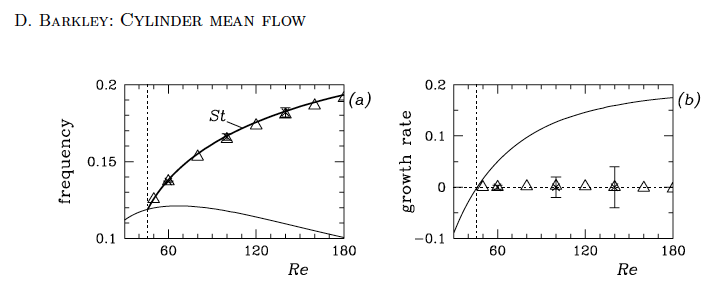
\includegraphics[width=8cm]{FIGURES/Barkley_figure.png}
%%$$
%
% 
% 
%% \ssp It has been remarked that stability analysis of the {\em mean flow} obtained by time-averaging the limit cycle gives better predictions (Barkley, Leontini,...).
%  
%  
%%\ssp 
%  
% % => Objective of nonlinear stability approaches : Give a rigourous ground to study the stability of mean flow.
%  
%  
%
%\end{frame}
%
%\begin{frame}{Weakly nonlinear approach {\small (Sipp \& Lebedev, 2007)}}
%
%Starting point : weakly non-linear expansion, with multiple scale method.
%
%$$
%\epsilon : \frac{1}{Re_c} - \frac{1}{Re} ; \quad \tau = \epsilon^2 t
%$$
%
%\begin{eqnarray}
%{\bf u} &=& {\bf u}_{bc} + \epsilon \left[ A_{wnl} (\tau) \hat{\bf u} e^{i \omega_c t} + c.c. \right] \label{WNL1}\\
%&+& \epsilon^2 \left[ {\bf u}_\epsilon + |A_{wnl}|^2  {\bf u}_{2,0} + \left(  A_{wnl}^2 {\bf u}_{2,2} e^{2 i \omega_c t} + c.c. \right) \right] + {\cal O}( \epsilon ^3)
%\nonumber
%\end{eqnarray}
%
%
%\end{frame}
%
%
%
%\begin{frame}{Self-Consistent approach {\small (Mantic-Lugo, Arratia \& Gallaire, 2014)}}
%
%Starting point : Pseudo-eigenmode decomposition
%
%
%
%\end{frame}



\section{The future of StabFem }

\begin{frame}{Recent progress}

\begin{itemize}

\item Multi-platform objective : 
MacOs OK ; Unix OK ; Windows 10 currently 50 \% compatible.

{\small main issues with windows : cp = copy,...}%  \verb|\| instead of \verb|/|,...}

\item Plotting options : recent intergration of "pdeplot2dff" from Markus "chloros" in place of pdeplot/pdetools .

{\small other solutions for plotting : tecplot converter, vtk converter, ...}

\item Compatibility with Octave : currently 50 \% compatible.

{\small Main issues with octave : importdata, plotting (now solved), inputParser (now solved)}.

\item Translation in Python  ??

\end{itemize}

\end{frame}




%%%%%%%%%%%%
\begin{frame}{Besoins}

\begin{itemize}

\item Maintaining a fully opensource  (Matlab-Octave or Python ?) and fully multiplatform version (windows).

\item Managing a list of test cases (non-regression tests, etc...)

\item Help simplifying/rationalizing the programation style.

\item Gestion of errors / debugging / "verbosity" ...

\item Upgrading to 3D / parallel computation ? (currently not priority)

\item Support with github  (/ gitlab ?)

\item Documentation 

Automatic generation from comments in programs ?  Doxygen ??


\end{itemize}


\end{frame}




\end{document}

